\section{Trazado de Conos con Vóxeles} % (fold)

\label{sec:trazado_de_conos_con_voxeles}

El proceso de trazado de conos con vóxeles funciona de manera similar a marcha de rayos o \emph{ray-marching}. La diferencia es que el volumen a muestrear por cada paso que da el rayo incrementa según la distancia al punto de origen del cono (ver Figura \ref{fig:vct_explain}). La forma del cono es esencialmente una discretización de un grupo de rayos trazados desde un punto en una superficie. Para obtener las muestras de volúmenes cada vez más grande se utilizan los niveles de \emph{mipmap} en la estructura de vóxeles.

\begin{wrapfigure}{l}{0.4\linewidth}
	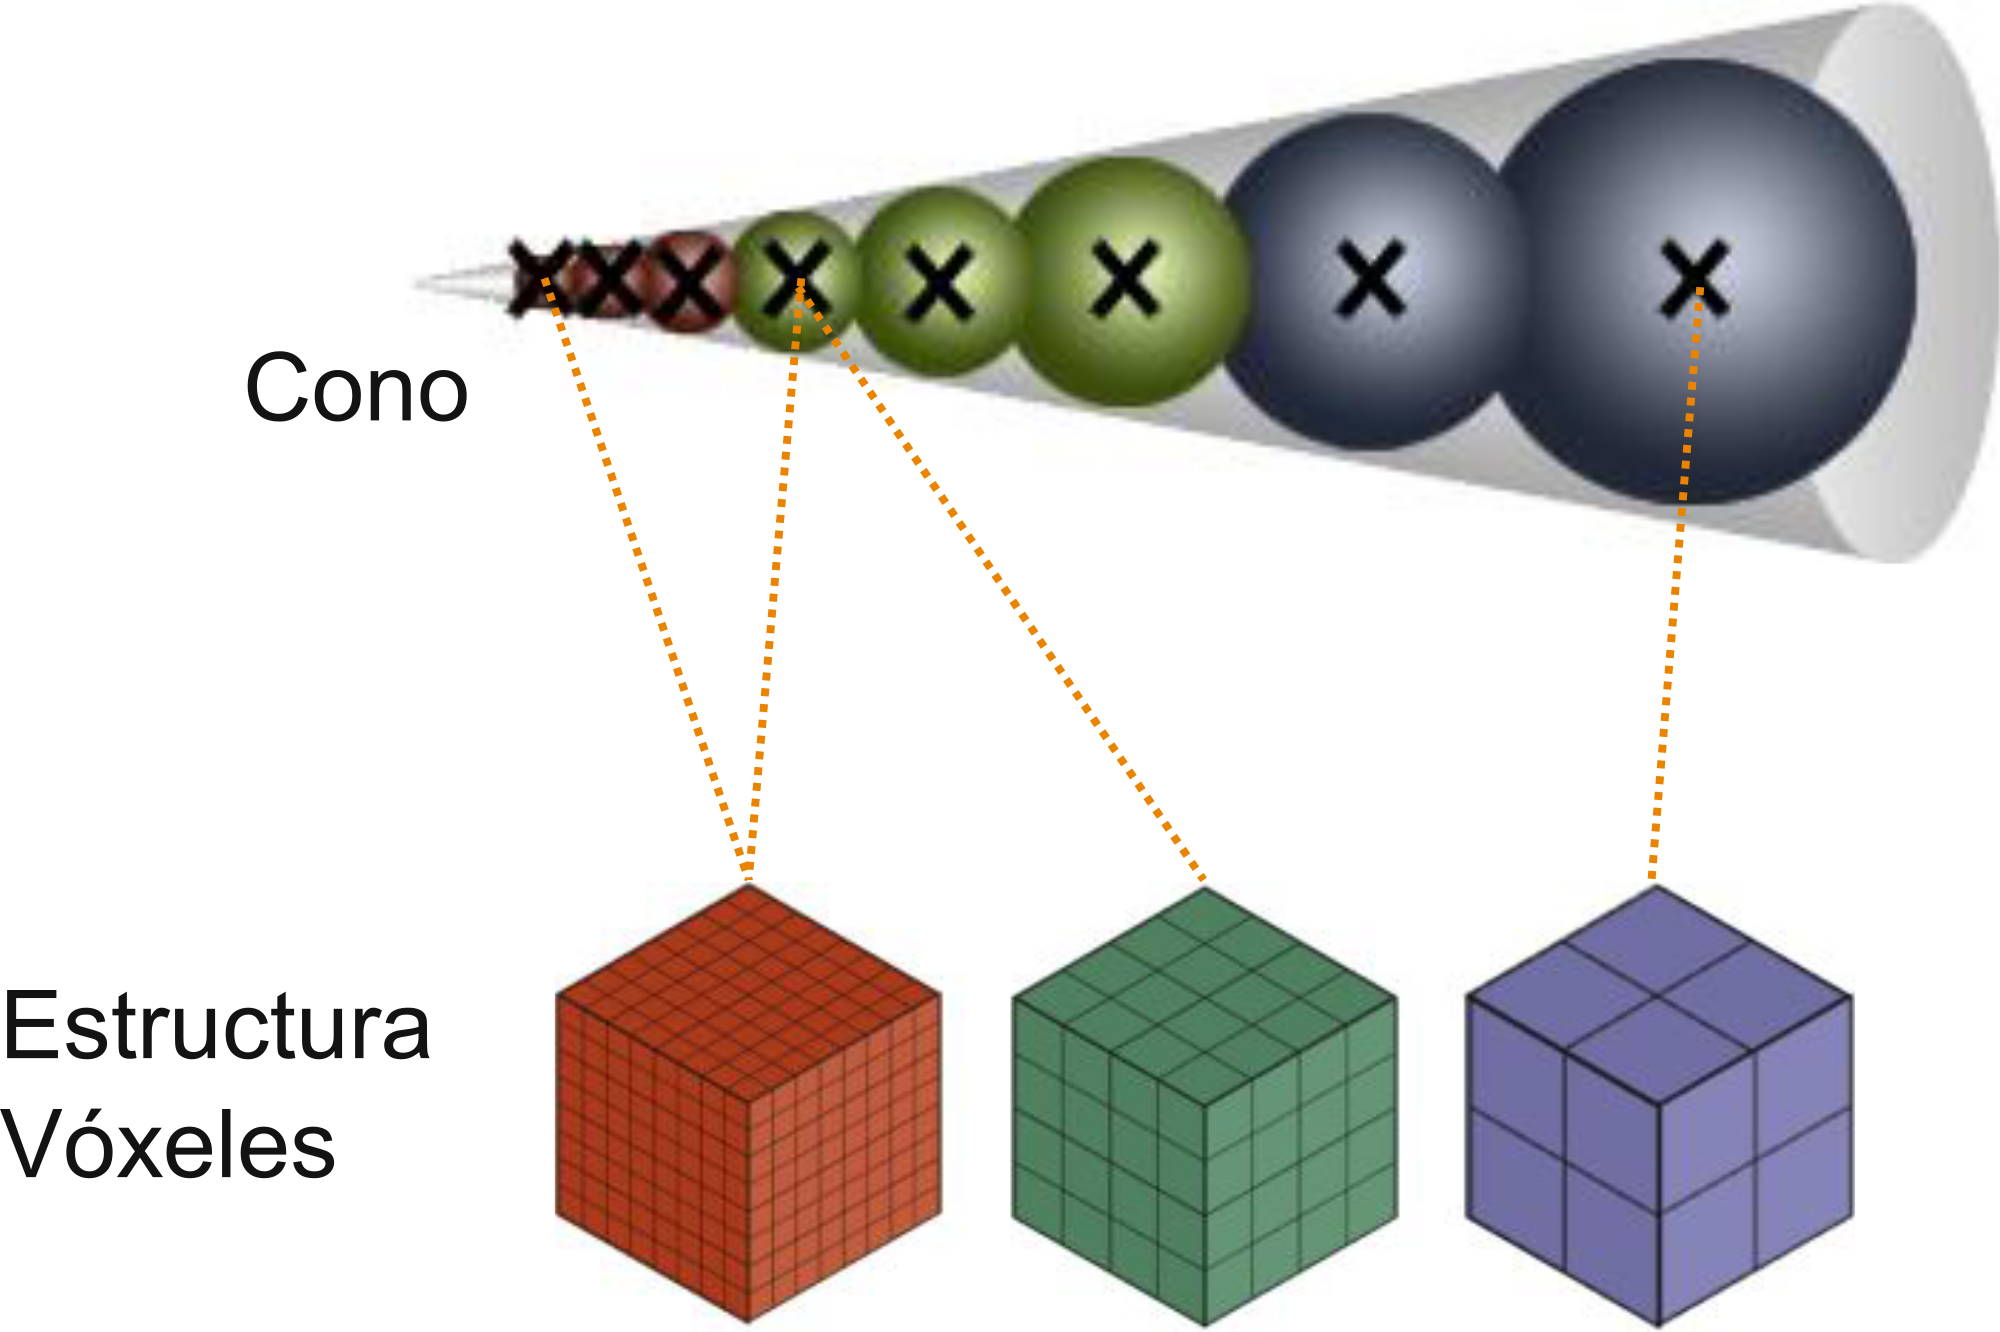
\includegraphics[width=0.95\linewidth]{media/vct_explain.png}
	\caption{Descripción gráfica del trazado de conos con vóxeles e interpolación entre distintos niveles de detalle \cite{Oliver:2012:UEE:2341836.2341909}.}
	\label{fig:vct_explain}
\end{wrapfigure}

\noindent Nuestra implementación realiza trazado de conos con vóxeles de la misma manera que fue explicada en la sección \ref{sub:voxel_cone_tracing_orig}, ya mayor diferencia reside en el uso de texturas 3D. Una de las principales ventajas de utilizar texturas 3D es que estas aceleran considerablemente el muestreo de la estructura jerárquica de vóxeles. Mientras que con un \emph{octree} cada vez que se desea trazar un cono el árbol tiene que ser recorrido de forma recursiva. Con texturas 3D esto se reduce a una simple instrucción proveída por OpenGL llamada \emph{textureLod}. Esta función recibe una textura, una coordenada de muestreo y un nivel de \emph{mipmap}. La función también realiza interpolación lineal entre los distintos niveles de \emph{mipmapping} si la textura a muestrear así lo habilita.
% section trazado_de_conos_con_voxeles (end)
\subsection{Reflexión Difusa}
La reflexión difusa de un fragmento puede ser aproximada utilizando integración Monte Carlo, trazando un número de conos sobre la semiesfera orientada por el vector normal del fragmento, y acumulando la radiancia a través del recorrido del cono. En nuestra implementación se utilizan seis conos difusos distribuidos de forma uniforme sobre la semiesfera (ver Figura \ref{fig:brdf_cones2}) orientada por el vector normal del fragmento.
\subsection{Oclusión Ambiental}
\label{sub:occl_ambt_prop}
La oclusión ambiental sobre un fragmento puede ser aproximada trazando conos sobre la semiesfera orientada por el vector normal de este. Para la oclusión ambiental solo es relevante acumular información de oclusión. El cono ambiental es ponderado por una función $f(r)$ donde su valor decae según la distancia recorrida. En nuestra aplicación se utiliza la función:
\begin{equation}
	f(r) = \frac{1}{1+\lambda r}
\end{equation} donde $r$ representa el radio del cono y $\lambda$ una variable personalizada que describe la intensidad de declive según la distancia para el término de oclusión ambiental, básicamente la extensión del radio de oclusión.
\subsection{Reflexión Especular}
Nuestra implementación utiliza como modelo de iluminación la \ac{BRDF} Blinn-Phong. Para obtener la reflexión especular es necesario solo un cono en equivalencia al lóbulo especular de la \ac{BRDF} como se observa en la Figura \ref{fig:brdf_cones2}. La apertura del cono especular depende del factor $n$ en Blinn-Phong, mientras más alto es este valor menor es la apertura del cono especular.
\begin{figure}[H]
	\centering
	\begin{subfigure}[t]{.32\linewidth}
		\centering
		\captionsetup{justification=centering}
		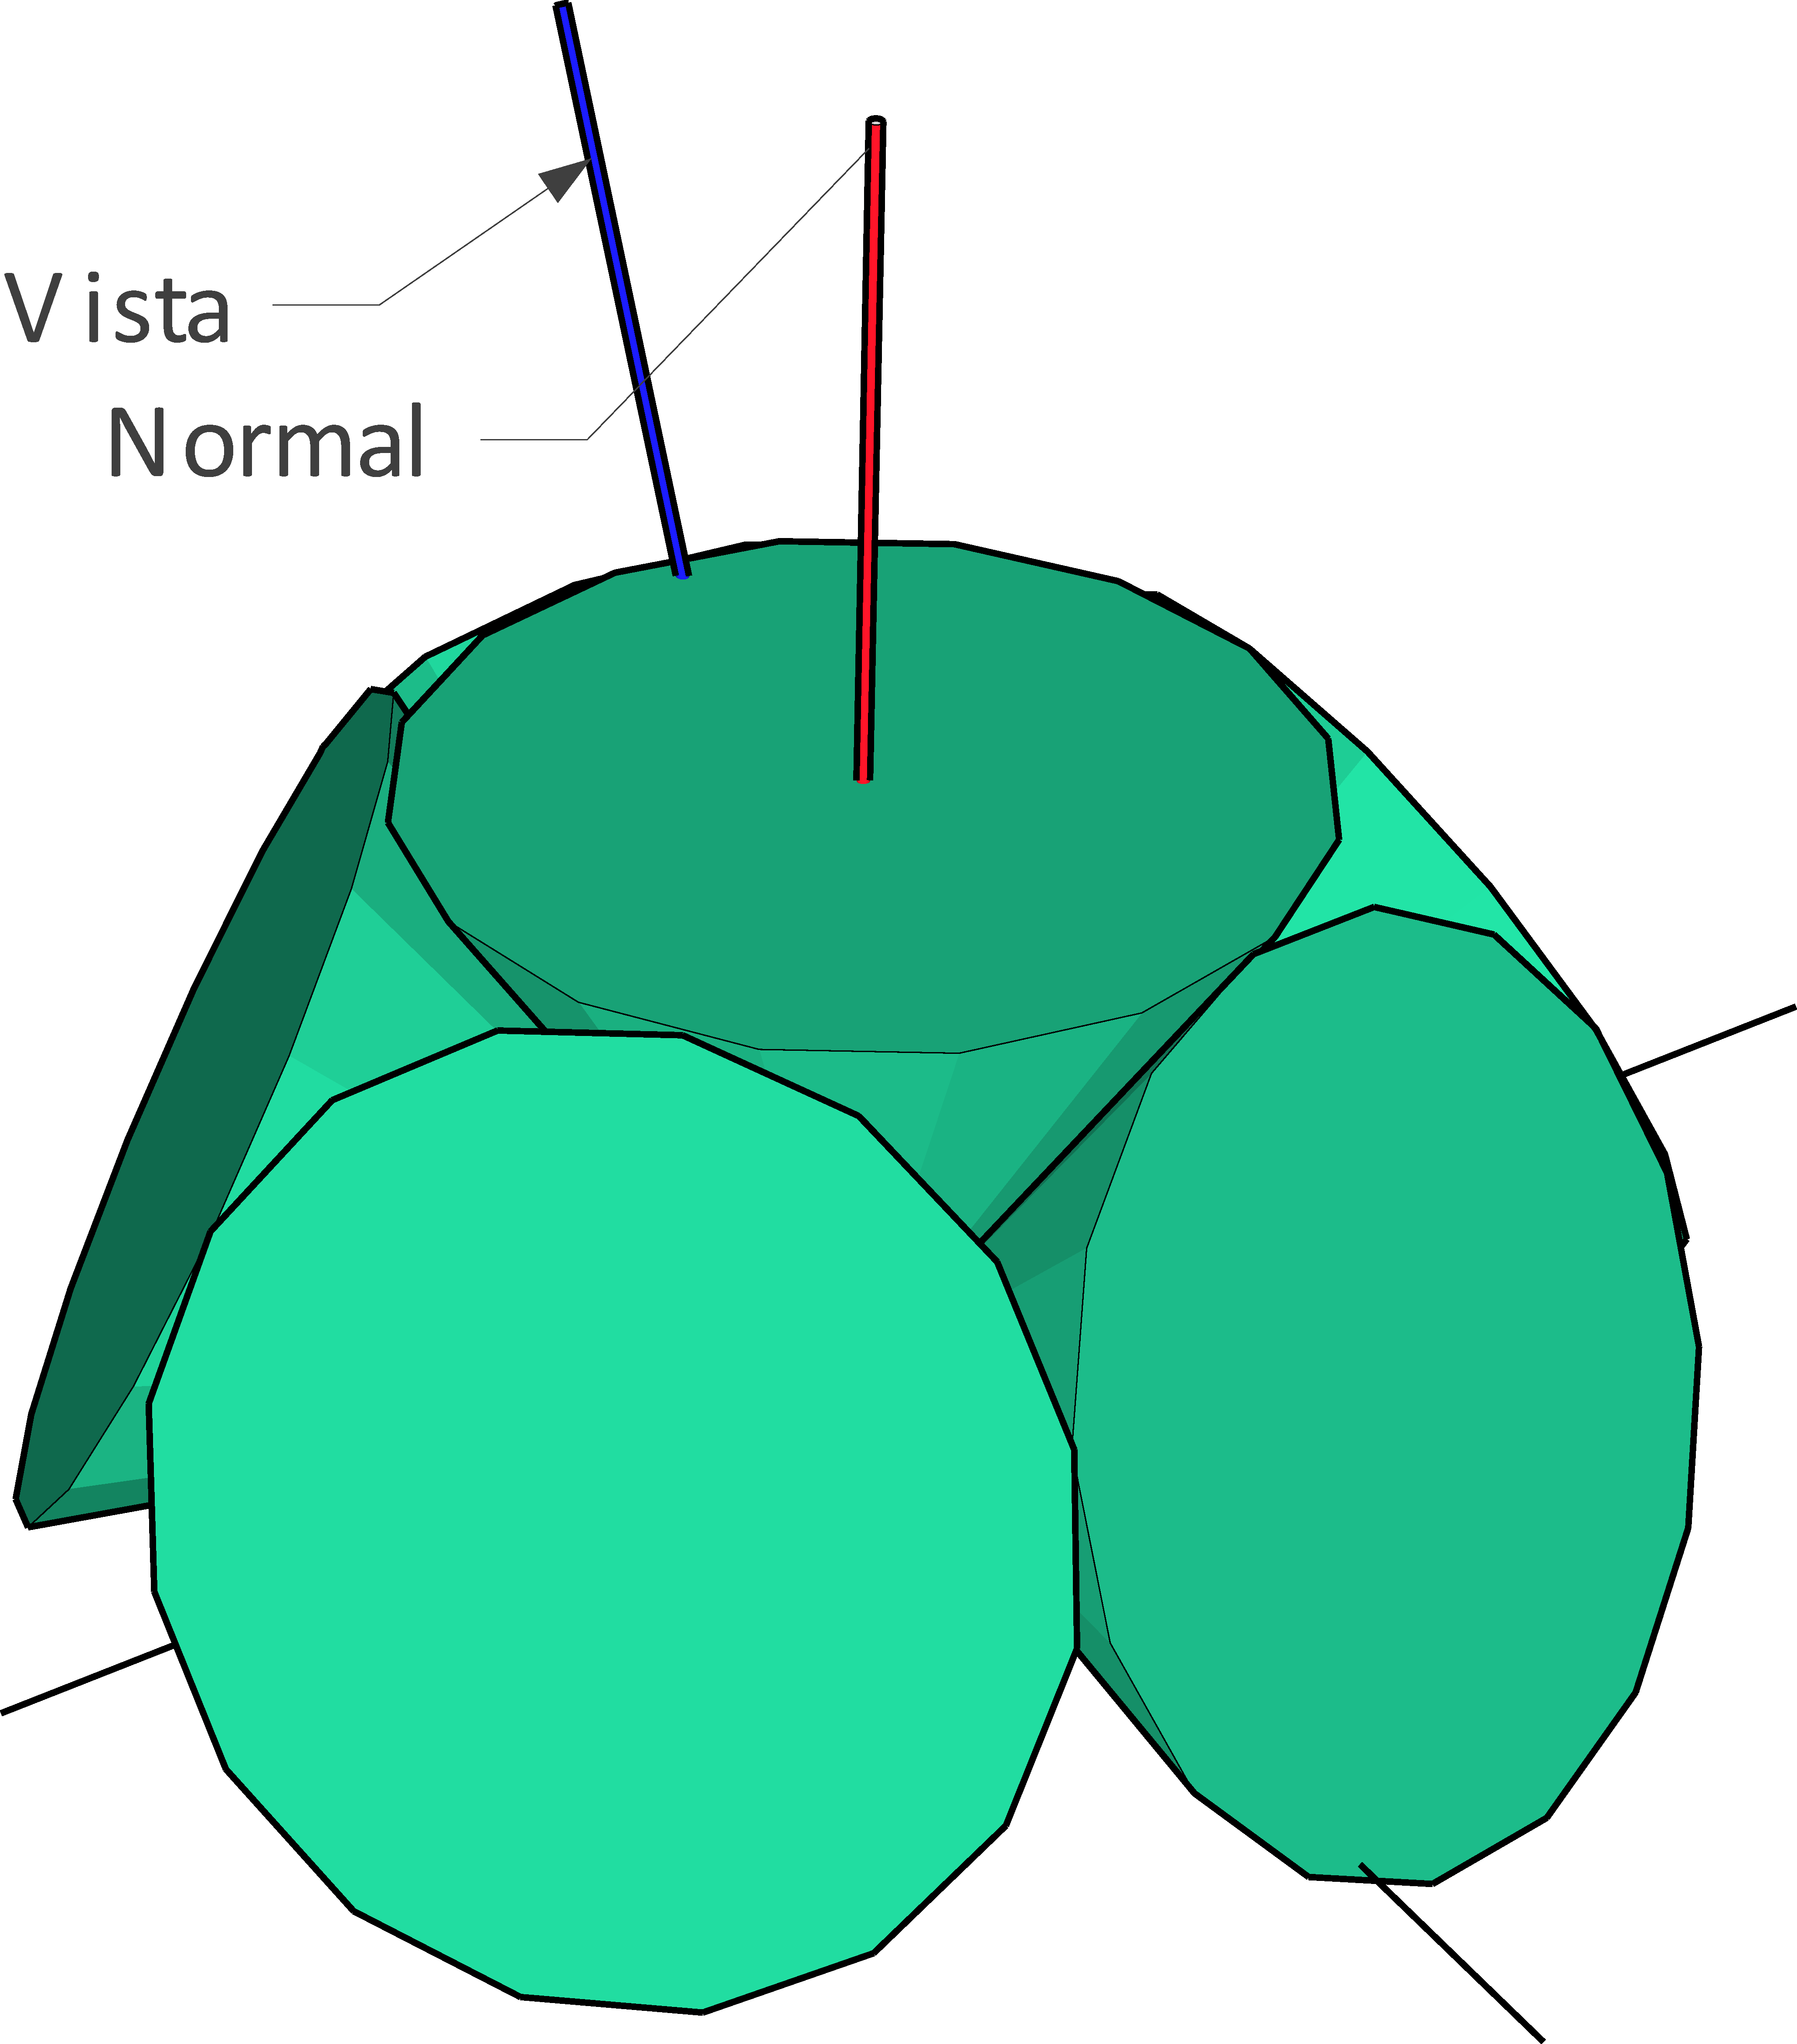
\includegraphics[width=\linewidth]{media/diffuse_cones_cropped.pdf}
		\caption*{Conos sobre la semiesfera para reflexión difusa.}
	\end{subfigure}%
	\hspace{0.01\textwidth}
	\begin{subfigure}[t]{.32\linewidth}
		\centering
		\captionsetup{justification=centering}
		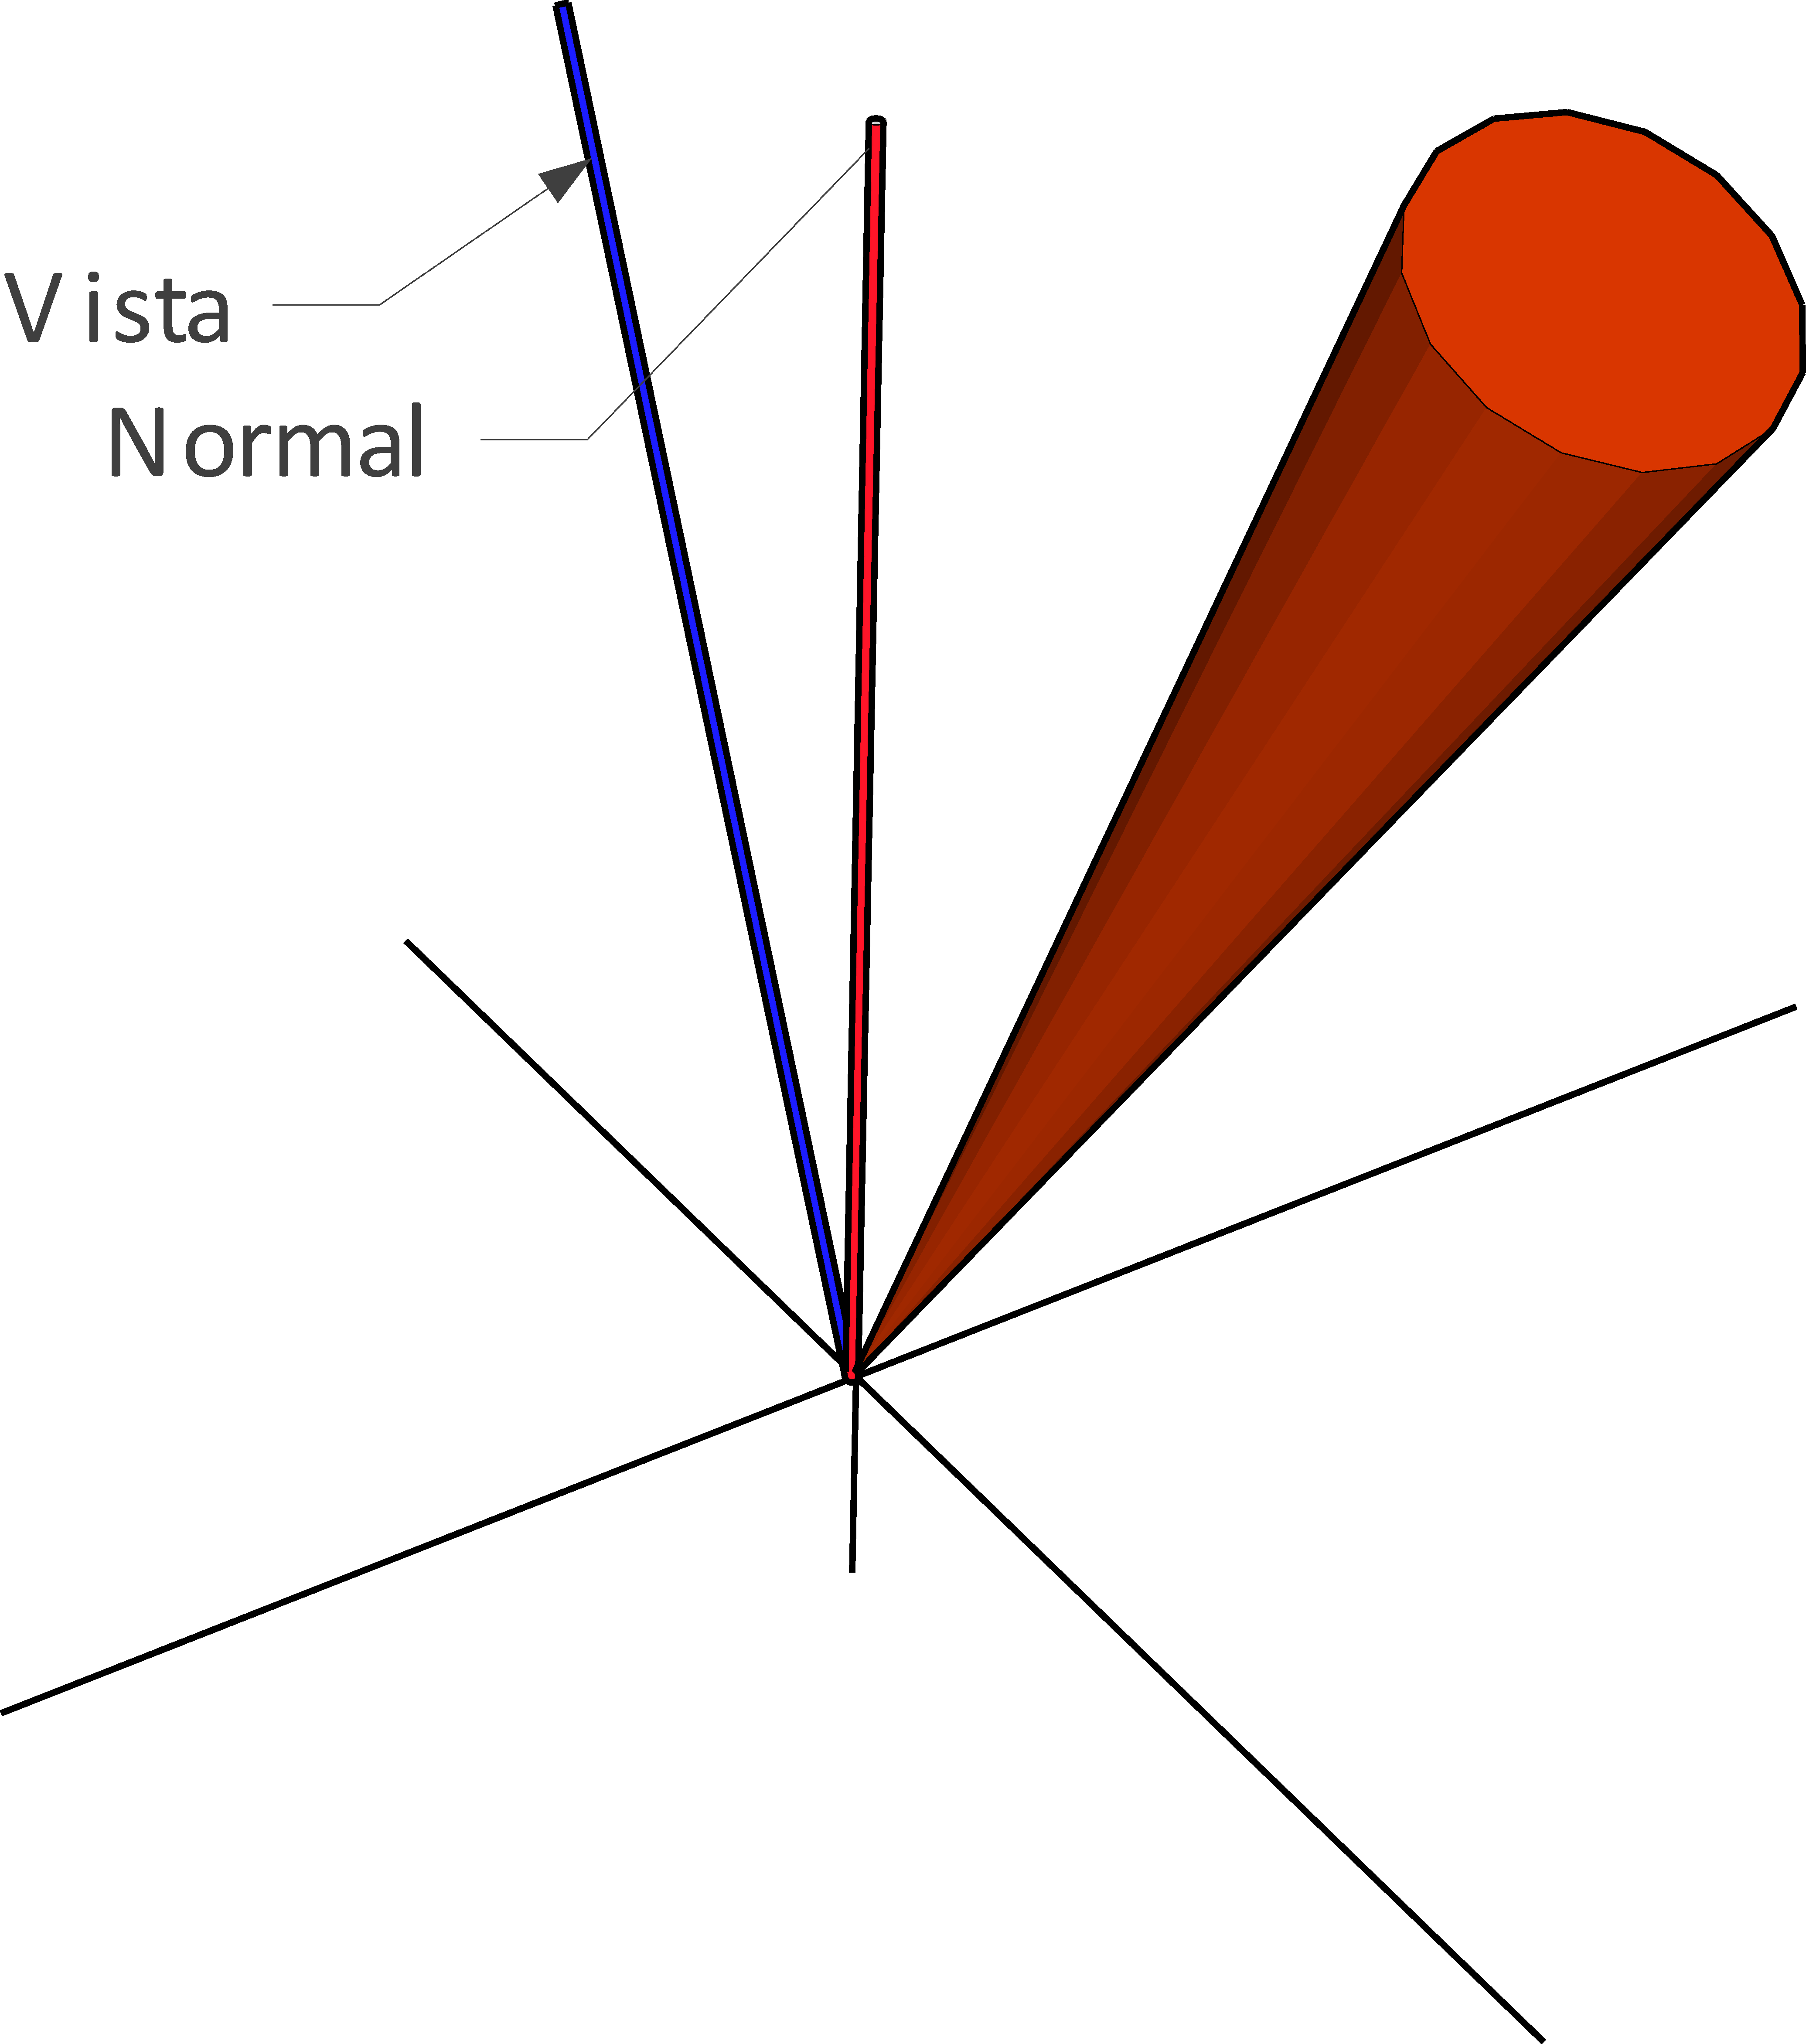
\includegraphics[width=\linewidth]{media/specular_cone_cropped.pdf}
		\caption*{Cono para el lóbulo especular.}
	\end{subfigure}%
	\hspace{0.01\textwidth}
	\begin{subfigure}[t]{.32\linewidth}
		\centering
		\captionsetup{justification=centering}
		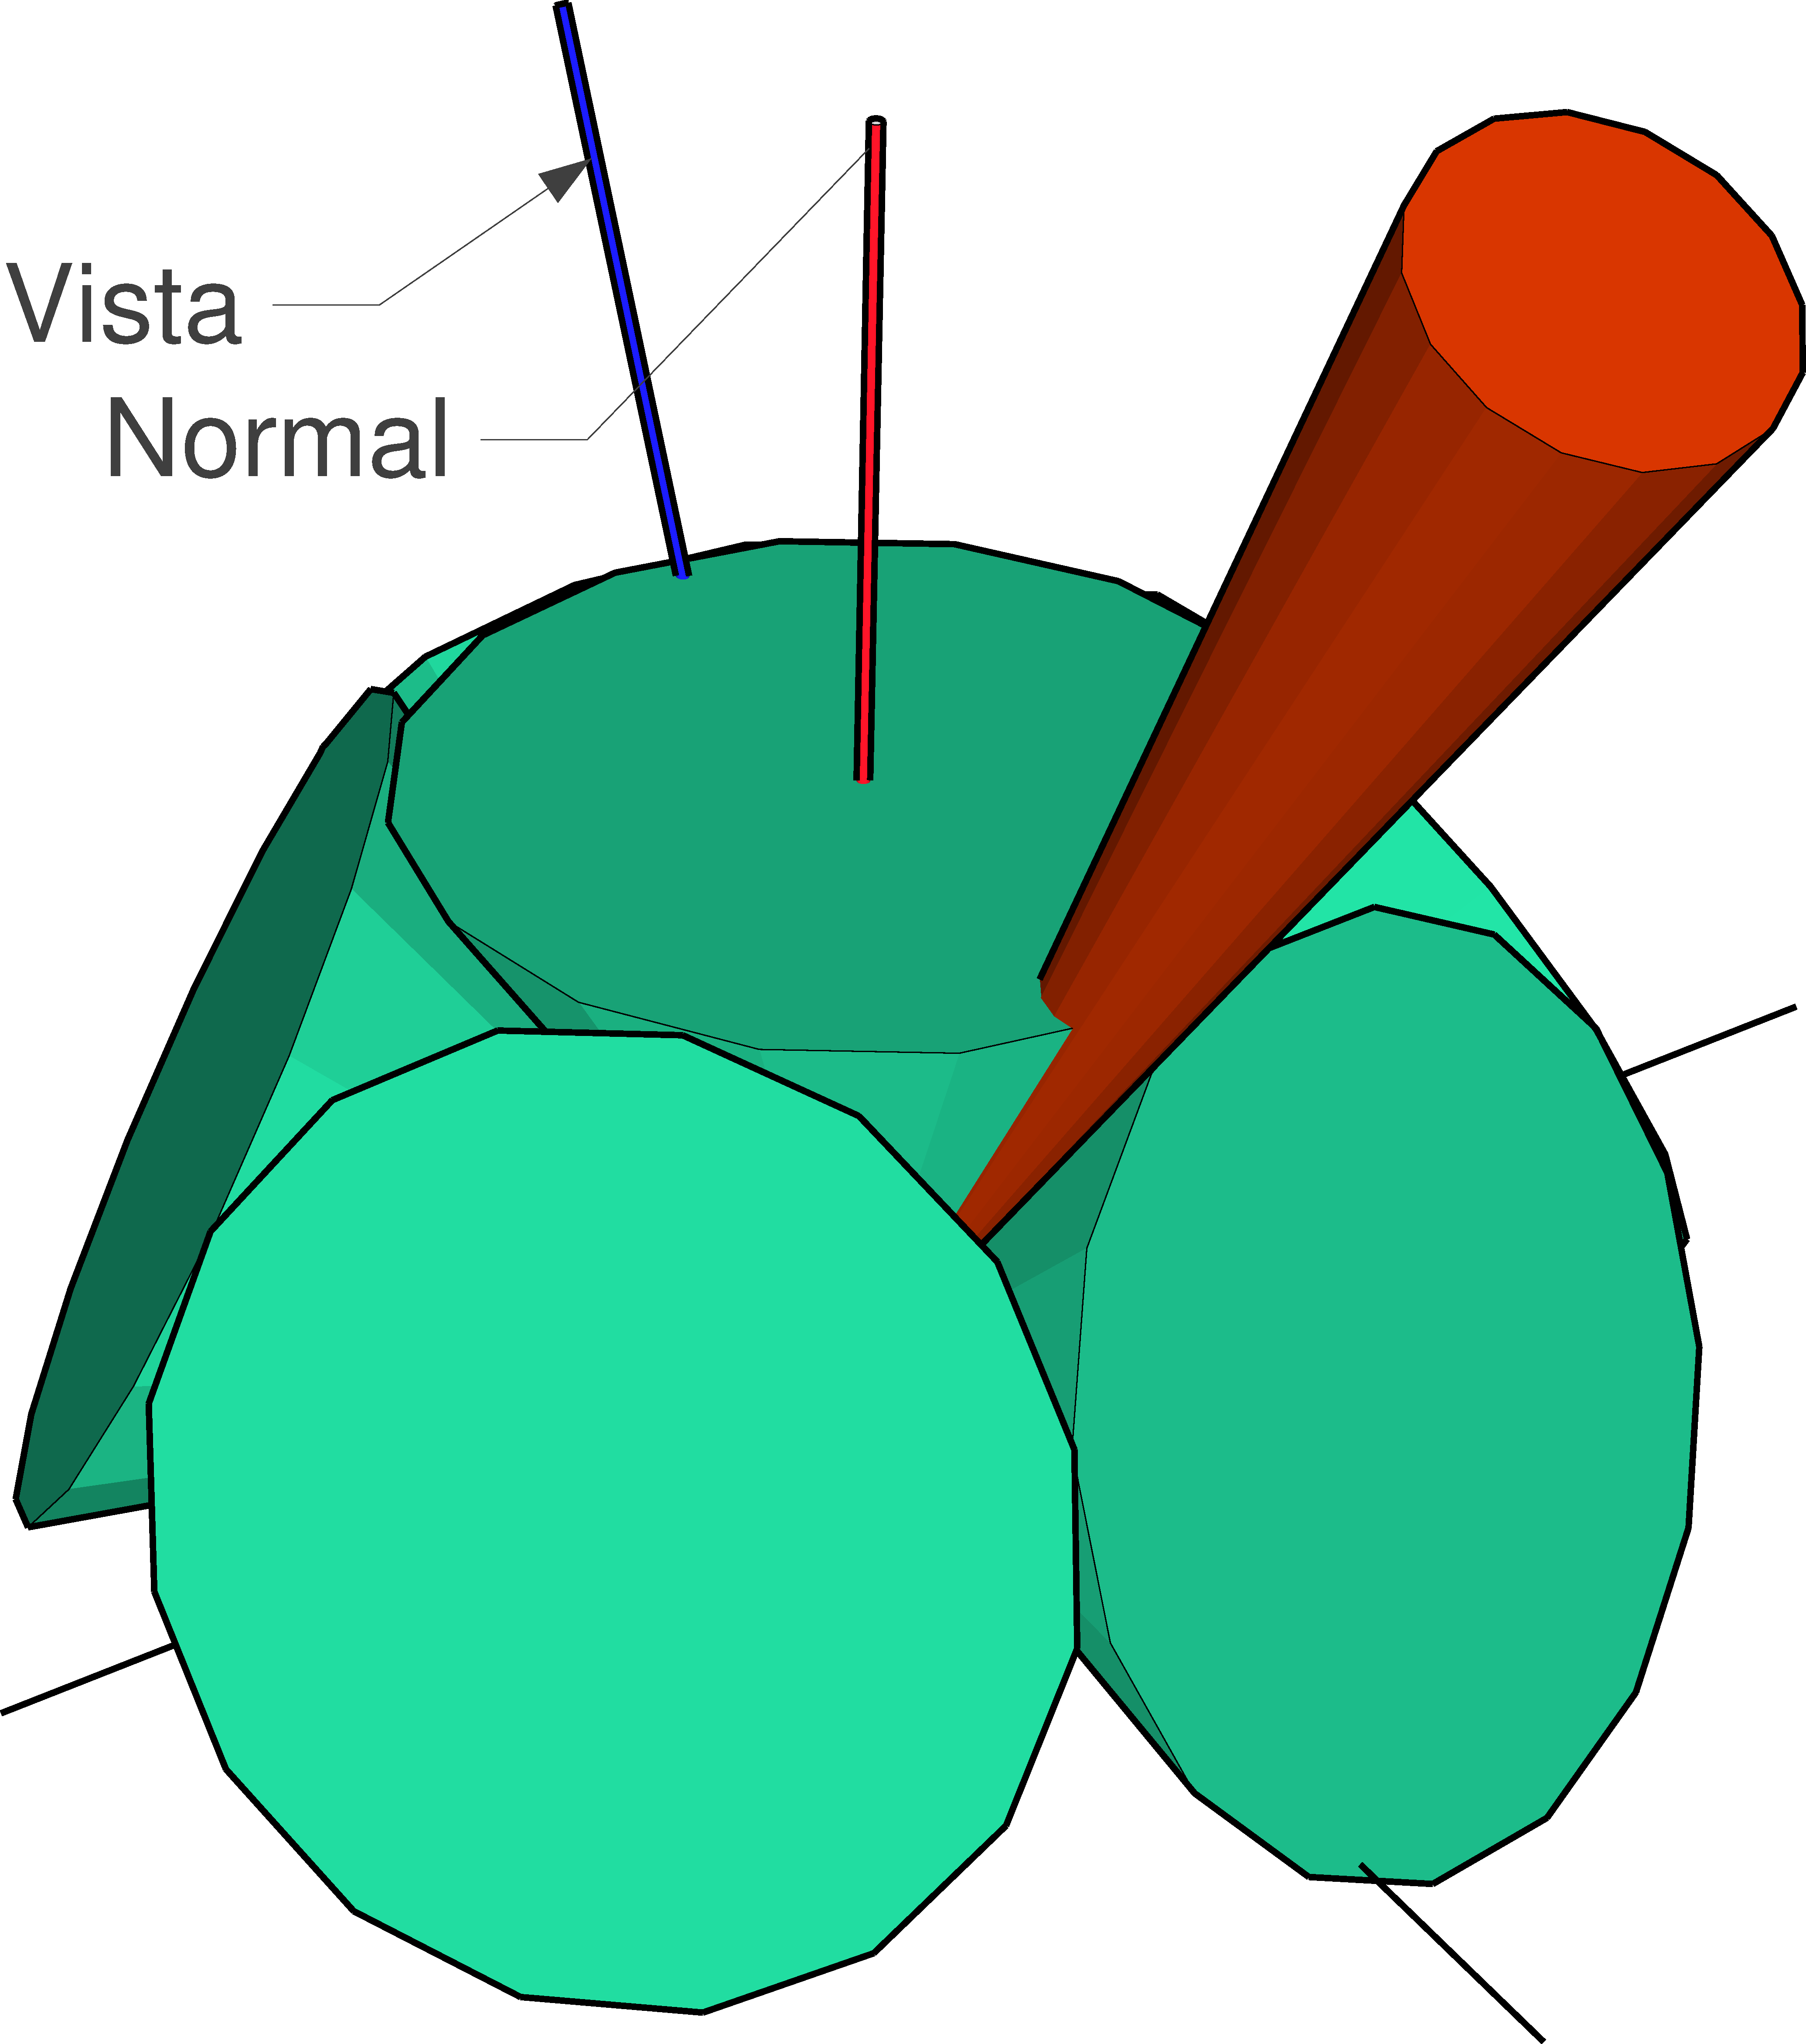
\includegraphics[width=\linewidth]{media/brdf_cones_cropped.pdf}
		\caption*{Discretización de la BRDF en conos.}
	\end{subfigure}%
	\caption{Ilustración de la distribución de los conos utilizados para representar la \ac{BRDF} Blinn-Phong.}
	\label{fig:brdf_cones2}
\end{figure}

\subsection{Sombras Suaves} % (fold)
\label{sub:sombras_suaves_con_trazado_de_conos}
El trazado de conos contra vóxeles también puede ser utilizado para realizar pruebas de oclusión sobre una superficie. En nuestra implementación se traza un cono desde la posición del fragmento en dirección opuesta a la dirección de la luz incidente. Para este cono se acumula la opacidad de los vóxeles. La apertura del cono permite controlar el umbral de la sombra resultante. A mayor apertura más suave y esparcida es la sombra. En la Figura \ref{fig:shadow_cone_prop} se describe el trazado de este cono.

\begin{figure}[H]
	\centering
	\captionsetup{justification=centering}
	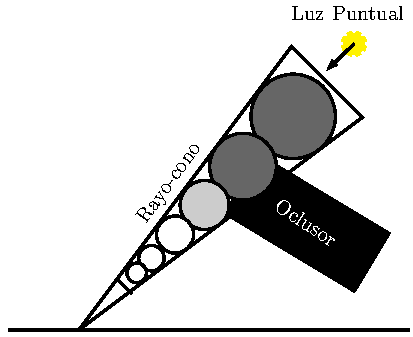
\includegraphics[width=.4\linewidth]{media/shadow_cone.pdf}
	\caption{Descripción gráfica del recorrido de un cono empleado para sombreado de superficies.}
	\label{fig:shadow_cone_prop}
\end{figure}

% subsection sombras_suaves_con_trazado_de_conos (end)
